% Historical source (removed by author request): references/_OLD_Übungsaufgaben/Übungsblatt 4 - Funktionen/Blatt4.tex:158
\begin{ExerciseBlock}
\ExerciseHeading{9}{Grenzwerte mit dem Einschließungsprinzip}{functions_squeeze_theorem}
Bestimmen Sie den Grenzwert
\begin{equation*}
	\lim_{x\rightarrow 0} \frac{\sin(x)}{x}.
\end{equation*}
\par\smallskip
Verwenden Sie, dass $\sin(x) \leq x \leq \tan(x)$ für $0<x<\pi/2$ gilt, und nutzen Sie dies, um den Nenner der zu untersuchenden Funktion abzuschätzen. Berücksichtigen Sie für den linksseitigen Grenzwert die Symmetrie von $\sin(x)/x$.

\begin{center}
	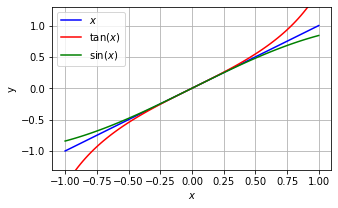
\includegraphics[width=0.6\textwidth]{content/resources/chapters/functions/images/squeeze_theorem.png} 
\end{center}

\end{ExerciseBlock}
\UseExerciseSolution{functions_squeeze_theorem}
